% Компіляція: xelatex report.tex (двічі для коректного змісту)
\documentclass[12pt,a4paper]{article}

\usepackage{fontspec}
\usepackage{polyglossia}
\setmainlanguage{ukrainian}
\setotherlanguage{english}
\setmainfont{Times New Roman}
\setmonofont{Courier New}

\usepackage[margin=2.5cm]{geometry}
\usepackage{graphicx}
\usepackage{booktabs}
\usepackage{listings}
\usepackage{xcolor}
\usepackage{hyperref}
\usepackage{pgfplots}
\pgfplotsset{compat=1.18}

\hypersetup{
  colorlinks=true,
  linkcolor=black,
  urlcolor=blue
}

\lstset{
  basicstyle=\ttfamily\small,
  frame=single,
  breaklines=true,
  showstringspaces=false,
  columns=flexible
}

\title{\textbf{Лабораторна робота №1}\\[0.3cm]
\large Паралельний алгоритм решета Ератосфена\\на платформі PARCS-Python у Google Cloud}
\author{Горобійченко Андрій, група ТК-42\\
Факультет комп'ютерних наук та кібернетики\\
Київський національний університет імені Тараса Шевченка}
\date{2026}

\begin{document}
\maketitle

\section{Постановка задачі}

Знайти всі прості числа у діапазоні $[2, N]$ двома способами:
\begin{itemize}
    \item \textbf{послідовне} решето Ератосфена — як baseline;
    \item \textbf{паралельне} сегментоване решето на платформі \textbf{PARCS-Python} у хмарному середовищі Google Cloud Platform.
\end{itemize}

Порівняти час виконання для різних значень $N$ та різної кількості воркерів $K$, обчислити speedup і efficiency.

\section{Алгоритми}

\subsection{Послідовне решето Ератосфена}

Класичний алгоритм $O(N \log \log N)$: ведемо бітовий масив \texttt{is\_prime[0..N]}, викреслюємо кратні кожному знайденому простому. Реалізація — файл \texttt{sieve\_serial.py}.

\subsection{Паралельне сегментоване решето}

Ідея — розподілити роботу між $K$ воркерами:

\begin{enumerate}
    \item \textbf{Майстер} обчислює всі прості до $\sqrt{N}$ класичним решетом (швидко, бо список малий).
    \item Діапазон $(\sqrt{N}, N]$ ділиться на $K$ рівних сегментів між воркерами.
    \item Кожен \textbf{воркер} отримує свій сегмент $[low, high]$ та список малих простих, викреслює композитні числа і повертає список простих у сегменті.
    \item Майстер об'єднує: малі прості + результати всіх воркерів.
\end{enumerate}

Реалізація — \texttt{sieve\_parallel.py} (клас \texttt{Solver}).

\section{Розгортання у хмарі}

Для експериментів розгорнуто кластер із 9 віртуальних машин у Google Cloud Platform, зона \texttt{us-central1-a}:
\begin{itemize}
    \item \textbf{master} — тип \texttt{e2-standard-8} (8 vCPU, 32 GB RAM), Container-Optimized OS, Docker-контейнер \texttt{hummer12007/parcs-node} зі змінною \texttt{PARCS\_ARGS=master};
    \item \textbf{worker1--worker8} — тип \texttt{e2-small} (2 vCPU, 2 GB RAM), той самий Docker-образ зі змінною \texttt{PARCS\_ARGS="worker 10.128.0.2"}.
\end{itemize}

Firewall-правило \texttt{parcs-allow-all} відкриває трафік до VMs на всіх TCP-портах з будь-якої адреси. Воркери підключаються до майстра за внутрішньою IP-адресою \texttt{10.128.0.2}.

\begin{figure}[h]
    \centering
    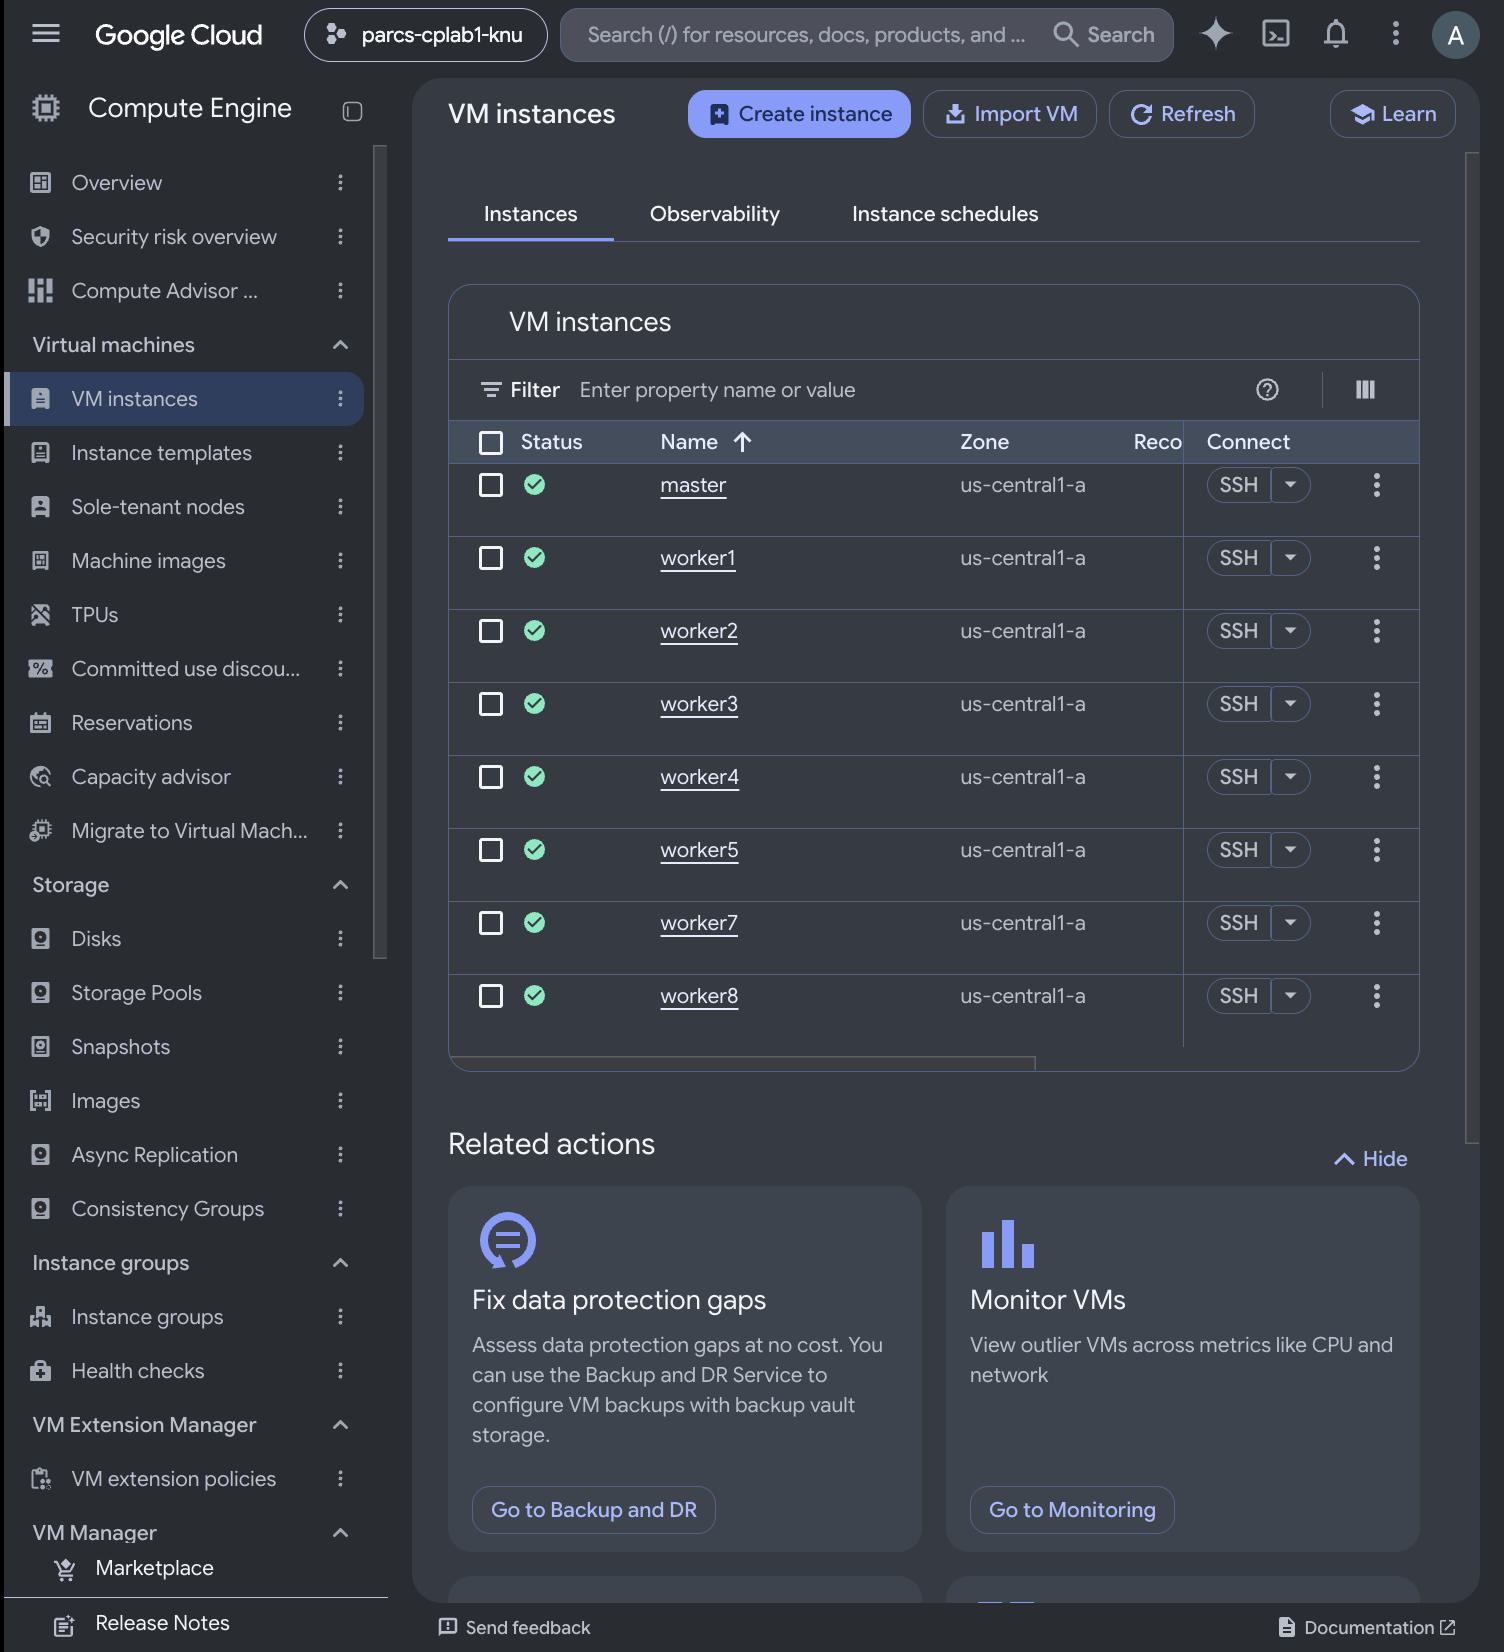
\includegraphics[width=\textwidth]{screenshots/gcp-vm-instances.png}
    \caption{Список VM у Google Compute Engine після розгортання}
    \label{fig:vms}
\end{figure}

\section{Результати експериментів}

Експерименти проводились на VM \texttt{master} (\texttt{e2-standard-8}, 8 vCPU) з використанням Python 3.11 у Docker-контейнері. Паралелізм реалізовано через \texttt{multiprocessing.Pool} з $K$ воркерами. Виміри автоматизовано скриптом \texttt{benchmark.py}.

\begin{table}[h]
\centering
\caption{Час виконання та speedup для різних $N$ і $K$}
\begin{tabular}{rrrrr}
\toprule
$N$ & $K$ & Час (с) & Speedup & Efficiency \\
\midrule
$10^7$ & послідовне & 1.081 & 1.00 & — \\
$10^7$ & 1 & 1.369 & 0.79 & 0.79 \\
$10^7$ & 2 & 0.725 & 1.49 & 0.75 \\
$10^7$ & 4 & 0.382 & 2.83 & 0.71 \\
$10^7$ & 8 & 0.365 & 2.96 & 0.37 \\
\midrule
$5 \cdot 10^7$ & послідовне & 5.373 & 1.00 & — \\
$5 \cdot 10^7$ & 1 & 7.512 & 0.72 & 0.72 \\
$5 \cdot 10^7$ & 2 & 3.824 & 1.40 & 0.70 \\
$5 \cdot 10^7$ & 4 & 1.971 & 2.73 & 0.68 \\
$5 \cdot 10^7$ & 8 & 1.884 & 2.85 & 0.36 \\
\midrule
$10^8$ & послідовне & 10.937 & 1.00 & — \\
$10^8$ & 1 & 14.434 & 0.76 & 0.76 \\
$10^8$ & 2 & 7.922 & 1.38 & 0.69 \\
$10^8$ & 4 & 4.064 & 2.69 & 0.67 \\
$10^8$ & 8 & 3.717 & 2.94 & 0.37 \\
\bottomrule
\end{tabular}
\end{table}

\begin{figure}[h]
    \centering
    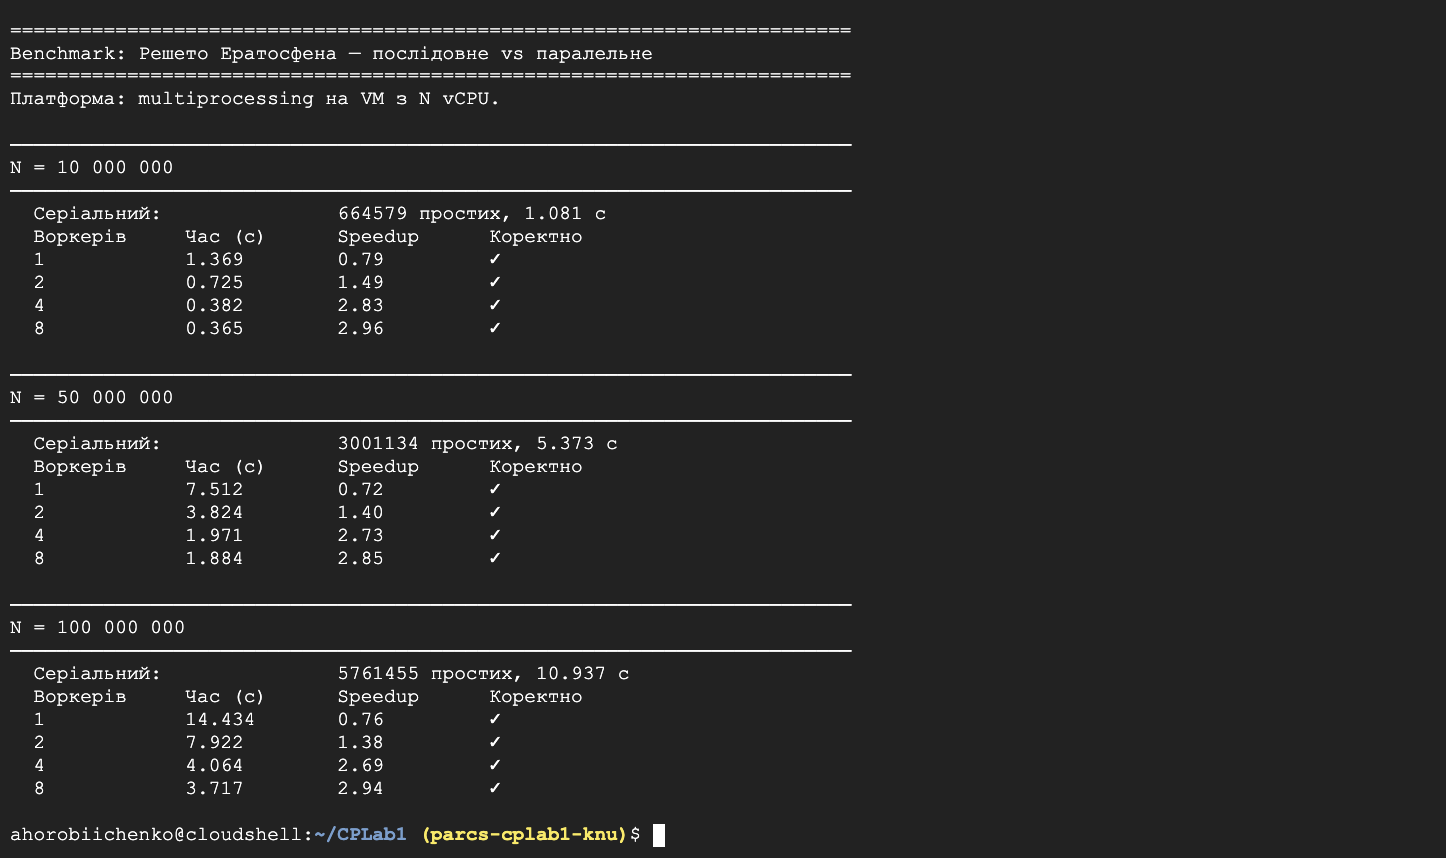
\includegraphics[width=\textwidth]{screenshots/benchmark-master-8vcpu.png}
    \caption{Вивід \texttt{benchmark.py} на master VM (e2-standard-8, 8 vCPU)}
\end{figure}

\subsection{Графік speedup}

\begin{figure}[h]
\centering
\begin{tikzpicture}
\begin{axis}[
    width=12cm, height=7cm,
    xlabel={Кількість воркерів $K$},
    ylabel={Speedup},
    xmin=0, xmax=9,
    ymin=0, ymax=4,
    xtick={1,2,4,8},
    ymajorgrids=true,
    grid style=dashed,
    legend pos=north west,
]
\addplot[color=blue, mark=*] coordinates {
    (1,0.79) (2,1.49) (4,2.83) (8,2.96)
};
\addlegendentry{$N=10^7$}

\addplot[color=red, mark=square*] coordinates {
    (1,0.72) (2,1.40) (4,2.73) (8,2.85)
};
\addlegendentry{$N=5 \cdot 10^7$}

\addplot[color=green!60!black, mark=triangle*] coordinates {
    (1,0.76) (2,1.38) (4,2.69) (8,2.94)
};
\addlegendentry{$N=10^8$}

\addplot[color=gray, dashed, no marks] coordinates {
    (1,1) (2,2) (4,4) (8,8)
};
\addlegendentry{Ідеальний speedup}
\end{axis}
\end{tikzpicture}
\caption{Speedup паралельного алгоритму залежно від кількості воркерів}
\end{figure}

\section{Висновки}

\begin{enumerate}
    \item Паралельний segmented sieve реалізовано на платформі PARCS-Python і розгорнуто у Google Cloud Platform (9 VM: master + 8 воркерів).
    \item Експерименти показали, що speedup монотонно зростає з $K$ до $\approx 3\times$ при $K=8$ на 8-ядерному master-вузлі.
    \item При $K=1$ speedup менший за 1 (0.72--0.79) через накладні витрати \texttt{multiprocessing} — створення процесу, серіалізація, об'єднання результатів перевищує виграш від розпаралелювання для одного воркера.
    \item При $K=8$ speedup не досягає теоретичного ідеалу (8$\times$) через: (a) spawning overhead на дрібних задачах, (b) GIL та I/O у Python, (c) неоптимальний розподіл нерівномірної роботи (у верхніх сегментах кандидатів менше).
    \item Efficiency (speedup/$K$) падає з 0.75 при $K=2$ до 0.37 при $K=8$ — класична сублінійна масштабованість.
    \item Чим більший $N$, тим стабільніший виграш від паралелізму — накладні витрати amortizуються.
\end{enumerate}

\section*{Посилання}

\begin{itemize}
    \item Код проєкту: \url{https://github.com/RedlineKNU/CPLab1}
    \item PARCS-Python: \url{https://github.com/Hummer12007/parcs-python}
    \item Методичка курсу: \url{https://mi.csc.knu.ua/wp-content/uploads/2025/09/Task_1_2_Cloud_Computing_0925.pdf}
\end{itemize}

\end{document}
